%%%%%%%%%%%%%%%%%%%% book.tex %%%%%%%%%%%%%%%%%%%%%%%%%%%%%
%
% sample root file for the chapters of your "monograph"
%
% Use this file as a template for your own input.
%
%%%%%%%%%%%%%%%% Springer-Verlag %%%%%%%%%%%%%%%%%%%%%%%%%%


% RECOMMENDED %%%%%%%%%%%%%%%%%%%%%%%%%%%%%%%%%%%%%%%%%%%%%%%%%%%
\documentclass[pdftex,12pt, oneside]{article}

% choose options for [] as required from the list
% in the Reference Guide, Sect. 2.2
%\usepackage[paperwidth=8.5in, paperheight=13in]{geometry} % Folio
\usepackage[paperwidth=8.27in, paperheight=11.69in]{geometry} % A4

\usepackage{makeidx}         % allows index generation
\usepackage{graphicx}        % standard LaTeX graphics tool
                             % when including figure files
%\usepackage{multicol}        % used for the two-column index
\usepackage[bottom]{footmisc}% places footnotes at page bottom
\usepackage[english]{babel}
\usepackage{enumerate}
\usepackage{paralist}
\usepackage{float}
\usepackage{gensymb}  
\usepackage{listings}
%\usepackage{siunitx}
% etc.
% see the list of further useful packages
% in the Reference Guide, Sects. 2.3, 3.1-3.3
\renewcommand{\baselinestretch}{1.5}

\newcommand{\HRule}{\rule{\linewidth}{0.5mm}}

%\makeindex             % used for the subject index
                       % please use the style svind.ist with
                       % your makeindex program


%%%%%%%%%%%%%%%%%%%%%%%%%%%%%%%%%%%%%%%%%%%%%%%%%%%%%%%%%%%%%%%%%%%%%

\begin{document}

%\author{Priyanto Tamami}
%\title{BUKU PETUNJUK OPERASIONAL SISTEM INFORMASI GEOGRAFIS UNTUK PBB-P2 DENGAN MAPINFO VERSI 8.0}
%\date{22 Desember 2015}
%\maketitle

%\input{./01.title.tex}
\begin{center}
{\large PROPOSAL STUDI KELAYAKAN PENGOLAHAN DATA SISTEM BEA PEROLEHAN HAK ATAS TANAH DAN/ATAU BANGUNAN}
\\[1cm]
12 Maret 2016\\
Priyanto Tamami, S.Kom.
\end{center}

%\frontmatter%%%%%%%%%%%%%%%%%%%%%%%%%%%%%%%%%%%%%%%%%%%%%%%%%%%%%%

%\include{dedic}
%\include{pref}

%\include{02.pengesahan} 

%\tableofcontents
%\listoffigures

%\mainmatter%%%%%%%%%%%%%%%%%%%%%%%%%%%%%%%%%%%%%%%%%%%%%%%%%%%%%%%
%\include{part}
%\include{chapter}
%\include{chapter}
%\appendix
%\include{appendix}

%\include{03.konsep-sig}
%\include{04.pengenalan-software}
%\include{05.koordinat}
%\include{06.registrasi-transformasi-koordinat} 
%\include{07.digitasi-on-screen} 
%\include{08.query} 

%\backmatter%%%%%%%%%%%%%%%%%%%%%%%%%%%%%%%%%%%%%%%%%%%%%%%%%%%%%%%
%\include{solutions}
%\include{referenc}
%\printindex

%%%%%%%%%%%%%%%%%%%%%%%%%%%%%%%%%%%%%%%%%%%%%%%%%%%%%%%%%%%%%%%%%%%%%%

\section{LATAR BELAKANG MASALAH}

Setelah dilakukannya peralihan beberapa jenis pajak dari pusat ke daerah, maka daerah dituntut untuk lebih mandiri dalam penguatan atau peningkatan pendapatan asli daerah dari sisi pajak.

Beberapa alasan terjadinya pengalihan ini diantaranya yaitu :

\begin{enumerate}[1.]
  \item Memperluas objek pajak daerah dan retribusi daerah
  \item Menambah jenis pajak daerah dan retribusi daerah (termasuk diantaranya pengalihan PBB dan BPHTB menjadi pajak daerah)
  \item Memberikan diskresi penetapan tarif pajak kepada daerah
  \item Menyerahkan fungsi pajak sebagai instrumen penganggaran dan pengaturan pada daerah.
\end{enumerate}

Dengan kondisi demikian, maka pemerintah daerah harus dapat berkomunikasi langsung dengan masyarakat wajib pajak agar kebijakan kebijakan yang diambil lebih tepat dan lebih efektif.

Dari hal tersebut diatas maka diperlukan studi kelayakan apakah sebuah sistem informasi perlu dibangun dalam rangka tertib administrasi Bea Perolehan Hak Atas Tanah dan/atau Bangunan di Pemerintah Daerah Kabupaten Brebes.  

\section{MAKSUD DAN TUJUAN}

Maksud dan tujuan yang akan dicapai dalam kegiatan studi kelayakan ini yaitu menganalisa apakah aplikasi yang akan dikembangkan nantinya layak untuk dipublikasikan dan digunakan sebagai alat untuk melakukan administrasi pelayanan Bea Perolehan Hak atas Tanah dan Bangunan.

\section{BATASAN MASALAH}

Karena luasnya ruang lingkup dalam pembahasan studi kelayakan ini, maka penyusunan studi kelayakan akan diberikan batasan masalah bahwa Studi kelayakan ini melihat dari kebutuhan organisasi dalam hal ini instansi pemerintah terhadap suatu aplikasi berbasis web sebagai sarana berkomunikasi dengan masyarakat wajib pajak untuk jenis Pajak Bumi dan Bangunan Perdesaan dan Perkotaan sekaligus menjadi kontrol pembayaran pajak yang dititipkan wajib pajak atau kuasanya kepada pemerintah Desa untuk dibayarkan ke tempat pembayaran yang ditunjuk.
  
\section{PERENCANAAN TARGET}

%Target yang akan dicapai dari studi kelayakan ini melihat bahwa apakah kebutuhan pembuatan aplikasi web yang akan menampilkan informasi mengenai status pembayaran Surat Pemberitahuan Pajak Terhutang untuk jenis Pajak Bumi dan Bangunan Perdesaan dan Perkotaan, selain sebagai bentuk keterbukaan informasi kepada wajib pajak sekaligus sebagai kontrol terhadap petugas pemungut tingkat Desa/Kelurahan dalam menyalurkan realisasi penerimaan Pajak Bumi dan Bangunan Perdesaan dan Perkotaan dari wajib pajak atau kuasanya ke Bank Tempat Pembayaran, terhadap pemberlakuan kerahasiaan data wajib pajak pada Undang Undang Nomor 6 Tahun 1983 tentang Ketentuan Umum dan Tata Cara Perpajakan sebagaimana diubah terakhir dengan Undang Undang Nomor 16 Tahun 2009.

\section{PERSIAPAN PENGUMPULAN FAKTA}

%Dalam pengumpulan fakta pendukung studi kelayakan ini, karena dasarnya adalah kebutuhan organisasi terhadap beberapa ide dan melihat dari sisi hukum perpajakan yang berlaku, maka bentuknya adalah berupa survey internal mengenai setuju atau tidaknya membangun sebuah aplikasi sistem informasi status pembayaran Pajak Bumi dan Bangunan Perdesaan dan Perkotaan, serta dasar dasar hukum yang menyebutkan hal tentang kerahasiaan data wajib pajak.

\section{PENENTUAN JADWAL WAKTU}

%Penentuan jadwal waktu adalah sebagaimana tertera pada grafik gantt berikut ini :

%\begin{figure}[H]
%  \centering
%  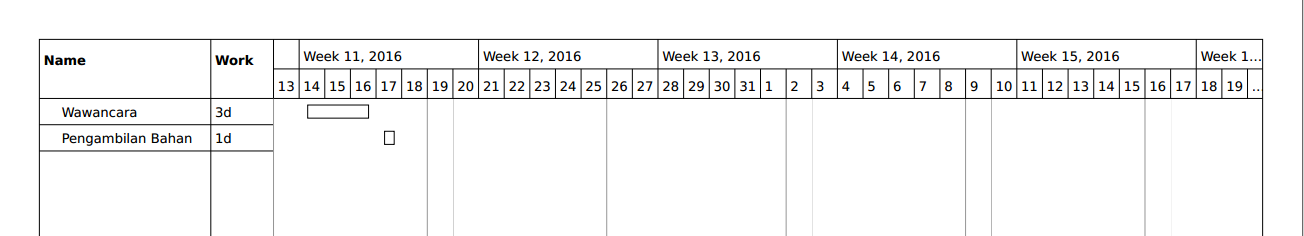
\includegraphics[width=0.7\textwidth]{./resources/jadwal-studi-kelayakan}
%  \caption{Jadwal Waktu Studi Kelayakan}
%\end{figure}

\section{CAKUPAN KEGIATAN}

%Cakupan kegiatan pada studi kelayakan ini hanya memerlukan pengumpulan hasil survey apakah aplikasi yang dibangun ini dianggap perlu atau tidak, serta melihat terhadap produk hukum, apakah aplikasi ini bertentangan atau tidak.

\section{TENAGA DAN BIAYA YANG DIPERLUKAN UNTUK STUDI KELAYAKAN}

%Tenaga yang diperlukan untuk studi kelayakan ini hanya 1 (satu) orang fungsional Pranata Komputer sebagai pengolah data hasil survey dan mempelajari aturan aturan mengenai ketentuan umum dan tata cara perpajakan, serta beberapa responden internal yang memberikan keterangan dalam lembar survey.

\end{document}